\documentclass[dissertation.tex]{subfiles}

\begin{document}

\begin{figure}[h]
    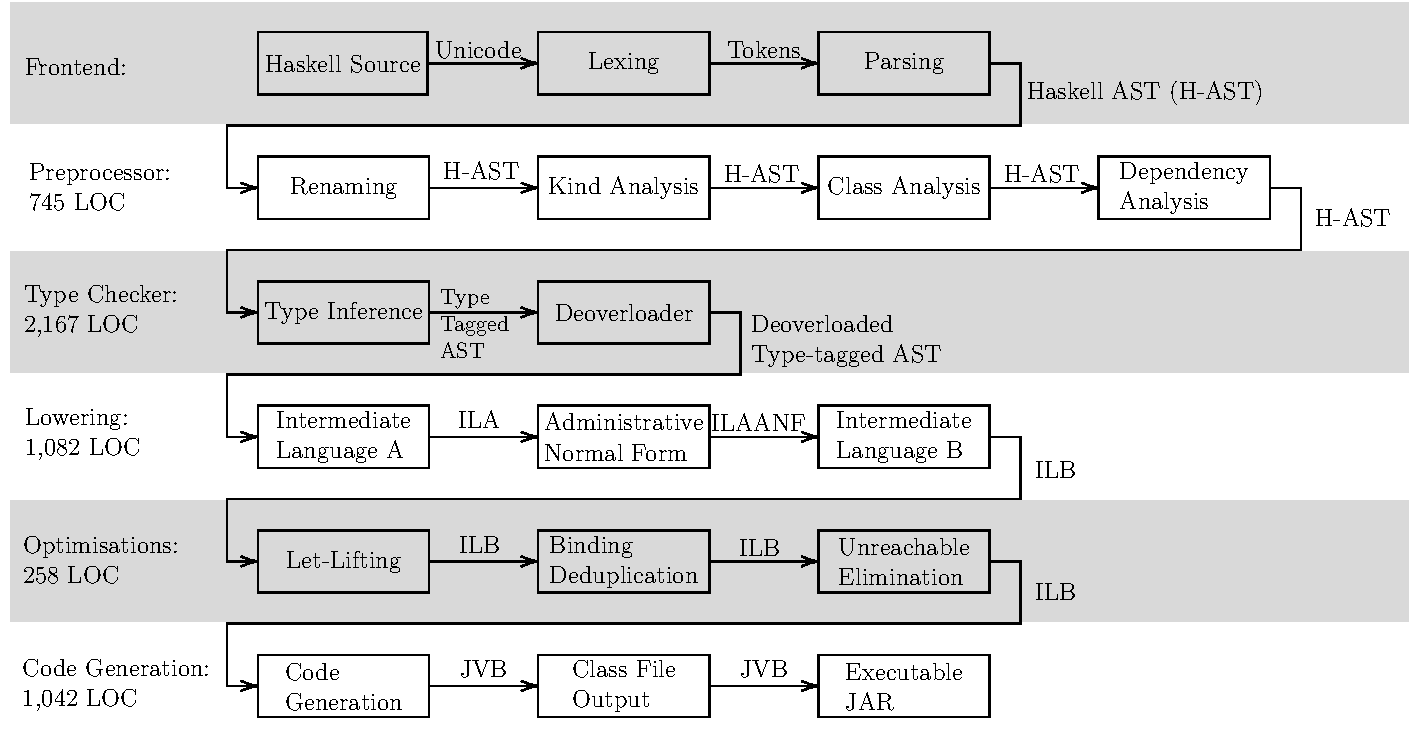
\includegraphics[width=\textwidth]{figures/compiler_layout.pdf}
    \caption{}
    \label{fig:compiler-layout}
\end{figure}

The compiler consists of a number of stages and substages, as shown in Figure \ref{fig:compiler-layout}. A brief overview of each stage was given in the preparation chapter (Section \ref{sec:compiler-structure}), but this chapter presents more in-depth descriptions. A summary is given at the end of the chapter, along with an overview of the code repository structure.

\section{Frontend}
{
    Lexing and parsing of Haskell source is performed using the \monospace{haskell-src}\footnote{https://hackage.haskell.org/package/haskell-src} library, which I modified to provide additional desirable features.

    The syntax supported by the frontend is a strict superset of Haskell 1998 and a strict subset of Haskell 2010, but \compilername does not support all of the features implied by the scope of the accepted syntax. For example, multi-parameter typeclasses are parsed correctly as a feature of Haskell 2010 but get rejected by the deoverloading stage.

    \begin{figure}[h]
        \begin{haskellfigure}
        class Convertable a b where
            convert :: a -> b
        instance Convertable Bool Int where
            convert True = 1
            convert False = 0
        \end{haskellfigure}
        \caption{An example of a multi-parameter typeclass}
    \end{figure}
}
\section{Preprocessor}
{
    The preprocessing passes either make the Haskell source easier to deal with by later passes, or extract useful information to prevent subsequent passes from needing to.

    \subsection{Renaming}
    {
        Haskell allows for multiple variables to share the same name within different scopes, which can increase the complexity of later stages in the pipeline. When typechecking the following code we might conflate the two uses of \haskell{x}, and erroneously infer that they have the same type. A similar problem arises with variable shadowing, when the scopes overlap. The problem also applies to any type variables present in the source -- the type variable \haskell{a} is distinct between the two type signatures:

        \begin{haskellfigure}
        id :: a -> a
        id x = x

        const :: a -> b -> a
        const x _ = x
        \end{haskellfigure}

        Additionally, variables and type variables are in different namespaces: the same token can refer to a variable and a type variable, even within the same scope. The following code is perfectly valid (but loops forever), despite the same name being used for a type variable and a variable:

        \begin{haskellfigure}
        x :: x
        x = x
        \end{haskellfigure}

        To eliminate the potential for subtle bugs stemming from this feature, the renamer pass gives each distinct variable/type variable in the source a unique name (in the above example, the variable \haskell{x} might be renamed to \haskell{v0} and the type variable renamed to \haskell{tv0}, provided those names have not already been used).
        
        The renamer traverses the syntax tree maintaining a mapping from a syntactic variable/type variable name to an associated stack of unique semantic variable names (in Haskell, a \haskell{Map VariableName [UniqueVariableName]}):

        \begin{itemize}
        \item When processing the binding site of a new syntactic variable (eg.\ a let binding, a lambda argument, a pattern match...), a fresh semantic name is generated and pushed onto the stack associated with the syntactic variable.
        \item Whenever we leave the scope of a syntactic variable, we pop the top semantic name from the associated stack.
        \item When processing a use site of a syntactic variable, we replace it with the current top of the associated stack.
        \end{itemize}

        An analogously constructed mapping is maintained for type variables, but is kept separate from the variable mapping: otherwise the keys can conflict in code such as \haskell{x :: x}.

        Type constants such as \haskell{Bool} from \haskell{data Bool = False | True} and typeclass names like \haskell{Num} from \haskell{class Num a where ...} are not renamed: these names are already guaranteed to be unique by the syntax of Haskell, and renaming them would mean we need to maintain more mappings and carry more state through the compiler as to what they were renamed to.
    }
    \subsection{Kind/Class Analysis}
    {
        The typechecker and deoverloader require information about the kinds of any type constructors and the methods provided by different classes. This is tricky to compute during typechecking as those passes traverse the AST in dependency order. Instead, we just perform a traversal of the AST early in the pipeline to aggregate the required information. 
    }
    \subsection{Dependency Analysis}\label{sec:dependency-analysis}
    {
        When typechecking, the order of processing declarations matters: we cannot infer the type of \haskell{foo = bar baz} until we have inferred the types of \haskell{bar} and \haskell{baz}. The dependency analysis stage determines the order in which the typechecker should process declarations. 

        We compute the sets of free/bound variables/type variables/type constants for each declaration, then construct a dependency graph -- each node is a declaration, with an edge from \(A\) to \(B\) if any bound variables/type variables/type constants at \(A\) are free in \(B\). It is important to distinguish between variables/type variables and type constants, as otherwise name conflicts could occur (as type constants are not renamed). This separation is upheld in the compiler by using different types for each, and is represented in the dependency graph in Figure \ref{fig:dependency-graph} by colouring variables red and constants blue.

        The strongly connected components (SCCs) of the dependency graph correspond to sets of mutually recursive declarations, and the partial order between components gives us the order to typecheck each set. The compiler uses an existing Haskell library to compute the SCCs (\texttt{containers}\footnote{\url{https://hackage.haskell.org/package/containers}}), which uses the algorithm presented by M. Sharir\cite{SCC}.

        For example, from the dependency graph in Figure \ref{fig:dependency-graph} we know that: we need to typecheck \(d_3\), \(d_4\), and \(d_5\) together as they are contained within the same strongly-connected component so are mutually recursive; we have to typecheck \(d_2\) last, after both other components.

        \begin{figure}[h]
        \centering
        \begin{subfigure}[t]{0.4\textwidth}
            \begin{haskellfigure*}{linenos=false}
            data Bool = False | True      #\(d_1\)#
            x = f True                    #\(d_2\)#
            f y = g y                     #\(d_3\)#
            g y = h y                     #\(d_4\)#
            h y = f y                     #\(d_5\)#
            \end{haskellfigure*}
        \end{subfigure}
        \begin{subfigure}[t]{0.5\textwidth}
            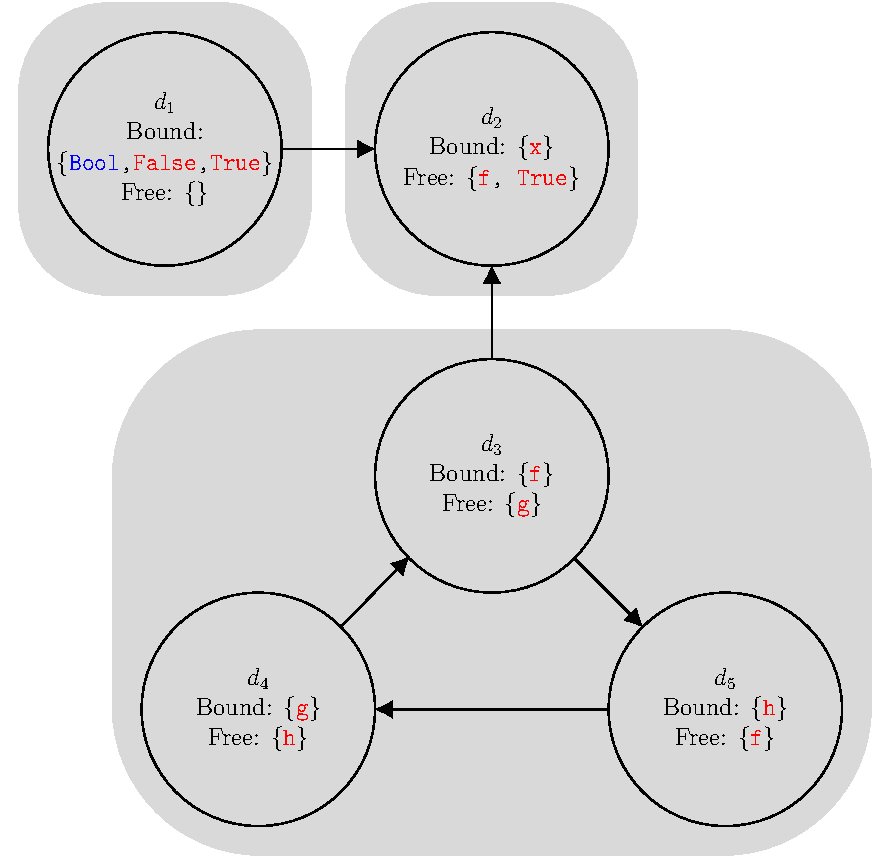
\includegraphics[width=\textwidth, valign=t]{figures/dependency_graph.pdf}
        \end{subfigure}
        \caption
        {
            Code labelled with declaration numbers, and the corresponding dependency graph. Variables are in red text, type constants in blue. Strongly connected components are highlighted.
        }
        \label{fig:dependency-graph}
        \end{figure}

        Typechecking declarations within the same component can proceed in an arbitrary order, we just need to ensure that the all of the type variables for the names bound by the declarations are available while processing each individual declaration.

        \paragraph*{Special cases due to Typeclasses}

        This process given above works for languages without ad-hoc overloading, like SML. However, in Haskell there are some complications introduced by typeclasses:

        \begin{itemize}
        \item
        {
            Typeclass member variables can be declared multiple times within the same scope. For example:
            
            \begin{haskellfigure}
            class Num a where
                (+) :: a -> a -> a
            instance Num Int where
                x + y = ...
            instance Num Float where
                x + y = ...
            \end{haskellfigure}

            Here the multiple declarations of \haskell{(+)} do not conflict: this is a valid program. However, the following program does have conflicting variables, as \haskell{x} is not a typeclass member and is not declared inside an \haskell{instance} declaration:

            \begin{haskellfigure}
            x = True
            x = False
            \end{haskellfigure}

            These declaration conflicts can be expressed as a binary symmetric predicate on declarations, as presented in Figure \ref{fig:conflict-grid}, where:

            \begin{itemize}
            \item
            {
                \monospace{Sym #\(x\)#} and \monospace{Type #\(x\)#} represent top-level declaration and type-signature declarations for a symbol \(x\), like \haskell{#\(x\)# = True} and \haskell{#\(x\)# :: Bool}.
            }
            \item
            {
                \monospace{ClassSym #\(x\)# #\(c\)#} and \monospace{ClassType #\(x\)# #\(c\)#} represent \monospace{Sym #\(x\)#} and \monospace{Type #\(x\)#} inside the declaration for a class \(c\), like \haskell{class #\(c\)# where { #\(x\)# = True ; #\(x\)# :: Bool }}.
            }
            \item
            {
                \monospace{InstSym #\(x\)# #\(c\)# #\(t\)#} represents a \monospace{Sym #\(x\)#} inside the declaration for a class instance \(c\;t\), like \haskell{instance #\(c\)# #\(t\)# where { #\(x\)# = True }}.
            }
            \end{itemize}

            \begin{figure}[h]
            \small
            \setlength{\tabcolsep}{2pt}
            \begin{tabular}{ l | c c c c c }
            & \texttt{Sym} \(x_1\) & \texttt{Type} \(x_1\) & \texttt{ClassSym} \(x_1\) \(c_1\) &
            \texttt{ClassType} \(x_1\) \(c_1\) & \texttt{InstSym} \(x_1\) \(c_1\) \(t_1\) \\
            \hline
            \texttt{Sym} \(x_2\) & \(x_1=x_2\) & \texttt{False} & \(x_1=x_2\) & \(x_1=x_2\) & \(x_1=x_2\) \\
            \texttt{Type} \(x_2\) & & \(x_1=x_2\) & \(x_1=x_2\) & \(x_1=x_2\) & \(x_1=x_2\) \\
            \texttt{ClassSym} \(x_2\) \(c_2\) & & & \(x_1=x_2\) & \(x_1=x_2 \wedge c_1 \neq c_2\) & \(x_1=x_2 \wedge c_1
            \neq c_2\) \\
            \texttt{ClassType} \(x_2\) \(c_2\) & & & & \(x_1=x_2\) & \(x_1=x_2 \wedge c_1 \neq c_2\) \\
            \texttt{InstSym} \(x_2\) \(c_2\) \(t_2\) & & & & & \makecell{\(x_1=x_2 \wedge (c_1 \neq c_2 \vee t_1=t_2)\)}
            \\
            \end{tabular}
            \caption{The conflict relation: entries below the diagonal are omitted as the predicate is symmetric}
            \label{fig:conflict-grid}
            \end{figure}

            Using this table we can see that the multiple declarations for \haskell{(+)} in the example above are \monospace{InstSym (+) Num Int} and \monospace{InstSym (+) Num Float} so do not conflict, while the declarations for \haskell{x} above are both \monospace{Sym x} so do conflict.
        }
        \item\label{sec:dependencies-syntactic-semantic}
        {
            The dependencies generated by this technique are \textit{syntactic}, not \textit{semantic}: this is a subtle but important difference. The use of any ad-hoc overloaded variable generates dependencies on the class declaration that introduced the variable, but not the specific instance of the class that provides the definition of the variable used.

            \begin{haskellfigure}
            class Foo a where
                foo :: a -> Bool
            instance Foo Bool where
                foo x = x
            instance Foo [Bool] where
                foo xs = all foo xs
            \end{haskellfigure}

            The declaration of \haskell{foo} in \haskell{instance Foo [Bool]} semantically depends on the specific overload of \haskell{foo} defined in \haskell{instance Foo Bool}, and yet no dependency will be generated between the two instances as neither declaration binds \haskell{foo} (\haskell{foo} is treated as being free within the declarations as described above): they will only generate dependencies to \haskell{class Foo a} (and to the declaration of \haskell{Bool} and \haskell{all}).

            Computing the true semantic dependency graph is too complicated to be done in this pass, so the problem is left and instead solved during the typechecking stage using a just-in-time processing approach.
        }
        \end{itemize}

        To briefly summarise dependency analysis:

        \begin{itemize}
        \item Dependency analysis is required by typechecking in order to process declarations in the right order.
        \item
        {
            The ordering between strongly connected components of the dependency graph corresponds to the order in which to process declarations, to ensure that all dependent declarations have been processed already.
            
            The components themselves correspond to mutually recursive functions that need to be typechecked `together'.
        }
        \item Typeclasses introduce some interesting special cases to the otherwise intuitive process.
        \end{itemize}
    }
}
\section{Type Checker}
{
    Type inference and checking is the most complex part of the compiler pipeline. The type system implemented is approximately System \(\text{F}_\omega\) (the polymorphically typed lambda calculus with type constructors) along with algebraic data types, and type classes to provide ad-hoc overloading. The approximation is due to a number of restrictions made by the Haskell Report to ensure that type inference is decidable.
    
    This is a subset of the type system used by GHC (System \(\text{F}_\text{C}\)), which provides extensions such as GADTs and type families requiring a more complex type system.

    \subsection{Definition of Types}
    {
        \begin{haskellfigure}
        data TypeVariable = TypeVariable TypeVariableName Kind
        data TypeConstant = TypeConstant TypeVariableName Kind

        data Type = TypeVar TypeVariable
                  | TypeCon TypeConstant
                  | TypeApp Type Type Kind

        data Kind = KindStar
                  | KindFun Kind Kind
        \end{haskellfigure}

        Type variables have an associated kind\footnote{Kinds were described in the Preparation chapter, Section \ref{sec:kinds}.} to allow for type constraints such as \haskell{pure :: Functor #\(f\)# => #\(\alpha\rightarrow f \alpha\)#}, in which \haskell{f} has kind \(*\rightarrow*\).

        Note that function types (\(A \rightarrow B\)) are represented as applications of the \(\rightarrow\) type constructor. This simplifies logic in many places, as \(\rightarrow\) can usually be treated in the same way as type constructors like \haskell{Either}.

        \begin{haskellfigure}
        data TypePredicate = IsInstance ClassName Type

        data Qualified a = Qualified (Set TypePredicate) a
        type QualifiedType = Qualified Type

        data Quantified a = Quantified (Set TypeVariable) a
        type QuantifiedType = Quantified QualifiedType
        type QuantifiedSimpleType = Quantified Type
        \end{haskellfigure}

        A qualified/overloaded type is a simple type with type constraints/predicates attached, such as \haskell{Eq #\(\alpha\)# => #\(\alpha\rightarrow\alpha\rightarrow\)# Bool} (the type constraint here being just \haskell{Eq #\(\alpha\)#}). The type constraints act as restrictions on the valid types that can fulfil the type variable, or equivalently predicates which must hold on the variables: the type signature is only valid for \(\alpha\) that are instance of the \haskell{Eq} typeclass. 

        A quantified/polymorphic type is an overloaded type with a set of type variables that are universally quantified over the type, meaning they must later be instantiated to a specific type/type variable (universally quantified variables are `placeholder' variables). Haskell type signatures are implicitly quantified over all the contained type variables.

        During type inference, types are almost always polymorphic and often overloaded (\haskell{(==) :: forall #\(\alpha\)#. Eq #\(\alpha\)# => #\(\alpha\rightarrow\alpha\rightarrow\)# Bool}, \haskell{(+) :: forall #\(\alpha\)#. Num #\(\alpha\)# => #\(\alpha\rightarrow\alpha\rightarrow\alpha\)#}, \haskell{head :: [#\(\alpha\)#] -> #\(\alpha\)#}, ...). After deoverloading (Section \ref{sec:deoverloading}), types are never overloaded. This difference is enforced by using \haskell{QuantifiedType} and \haskell{QuantifiedSimpleType} respectively.
    }
    \subsection{Type Inference}
    {
        The implementation is inspired by the approach given by Mark P. Jones\cite{THIH} and uses similar rules as the Hindley-Milner (HM) type inference algorithm. There are three passes over the source AST, each of which traverses each SCC of the AST in dependency order as previously described in Section \ref{sec:dependency-analysis}.

        \begin{enumerate}
        \item
        {
            The first pass tags each subexpression of the declarations in the SCC with a type variable, then uses rules similar to the HM inference rules to infer the value of each type variable from subterm type variables.
            
            Overloaded functions present a difference from the HM rules, as some expressions generate typeclass constraints on the type variables involved: using an overloaded function like \haskell{(+)} will first require instantiating its polymorphic type to an overloaded type (\(\forall\alpha.\;\text{Num }\alpha\Rightarrow\alpha\rightarrow\alpha\rightarrow\alpha\) to \(\text{Num }\beta\Rightarrow\beta\rightarrow\beta\rightarrow\beta\), where \(\beta\) is a fresh unique type variable), then moving the constraints from the type into a set of constraints built up while traversing this declaration to get just \(\beta\rightarrow\beta\rightarrow\beta\). This is the ground type that is unified with the type variable used to tag the use of \haskell{(+)}, and the type constraints are stored for use after finishing traversing the SCC.

            After all declarations in an SCC have been fully traversed, types are generated for all the variable names bound. This involves adding explicit quantifiers and constraints to the simple type inferred for the top-level expression on the right-hand side of the binding. All type variables within the simple type that are not already in scope from eg.\ a class definition are added as universally quantified variables, and any constraints generated during processing the declaration involving type variables free in the simple type, are added as the qualifiers to the type.
        }
        \item
        {
            The second pass simply traverses the AST again and updates the tag type variables with the final expression type generated by the unification during the first pass.
            
            This cannot be done efficiently during the first pass as the final type is only known after fully traversing each SCC.
        }
        \item
        {
            The third pass checks that any user-provided type signatures are valid compared to what was actually inferred: if the user provided a more general tag than the inferred tag, we reject the program. This is distinct from the 3rd pass to maintain clarity.
        }
        \end{enumerate}

        An improvement to the current approach would be to implement the OutsideIn(X) framework given by Vytiniotis et al.\ \cite{OutsideIn}. This framework can work with Hindley-Milner type inference to handle more complex constraints than the current implementation, allowing support for GADTs and type families and handling type classes more flexibly than the current implementation.

        These three passes detail the inner workings, but there are still a number of tricky edge-cases to navigate:

        \subsubsection*{Restricted Polymorphism}
        {
            One departure from conventional polymorphic type systems is that Haskell's type system restricts polymorphism for some terms: let-bound variables are polymorphic over all their free type variables, while function parameters are never polymorphic. In practice, this means that in the code below, \haskell{f :: #\(\forall \alpha.\;\alpha \rightarrow \alpha\)#} whereas \haskell{g :: #\(\alpha \rightarrow \alpha\)#}. The difference in semantics ensures that type inference remains decidable. 

            \begin{haskellfigure}
            let f x = x in const (f True) (f 1) :: Bool -- This is fine
            (\g -> const (g True) (g 1)) (\x -> x)      -- This fails to typecheck
            \end{haskellfigure}
        }
        \subsubsection*{Typeclass Order}
        {
            A tricky part of the typechecking process is dealing with typeclasses, as dependency order is not semantically accurate for typeclass instance declarations: the problem is detailed in Section \ref{sec:dependencies-syntactic-semantic}.
            
            To handle the potential issues, such declarations are processed in a lazy manner. If a declaration requires an instance of a typeclass in order to typecheck then that typeclass is typechecked immediately, and all remaining instance declarations are processed after non-instance declarations have been processed.
        }
        \subsubsection*{The Ambiguity Check}
        {
            There is a type-system correctness check called the `ambiguity check', which ensures that at the use site of any variable with overloaded type has all type variables either resolved to a ground type or exposed in the type of the enclosing expression. This prevents programs which have ambiguous semantics (multiple possible runtime behaviours) from being reported as valid (this issue is described in Section 11.5.1 of `Typing Haskell in Haskell' \cite{THIH}). 

            My compiler does not implement this check, which causes some programs to fail compilation during the code generation stage instead of during typechecking. This feature was omitted in order to spend development time on the later stages of the compiler.

            Defaulting\footnote{\url{https://www.haskell.org/onlinereport/decls.html\#sect4.3.4}} is a user-friendly defence against the verbosity of giving unambiguous types. This feature was not implemented as the time required was expected to be better spent elsewhere.
        }
        \subsubsection*{Summary}
        {
            Having completed the three passes of type inference and checking, and handling the edge cases associated with typeclasses, the output of the type inference component is a Haskell AST where expressions are tagged with their (possibly overloaded) types. This forms the input for the final component before the compiler begins lowering the program into intermediate languages.   
        }
    }
    \subsection{Deoverloader}\label{sec:deoverloading}
    {
        The deoverloading stage performs a translation which implements typeclasses using a technique named dictionary passing. This produces an AST tagged with types that no longer have type contexts.

        \subsubsection{Dictionary Passing}
        {
            The expression \haskell{1 + 2} has type \haskell{Num a => a}, where the expression is `overloaded' on the type of \haskell{a} (as \haskell{(+)} is overloaded). This overloading can be implemented by adding extra parameters (`dictionaries') to all overloaded functions, which provide the implementation of any overloaded operators such as \haskell{(+)}. This is similar to virtual method tables in object oriented languages, except the v-table is being passed as an extrinsic argument, rather than being intrinsic to the object being operated on.

            Dictionary passing is implemented using a single source-to-source transformation on the Haskell AST:
            
            \begin{enumerate}
            \item
            {
                Each typeclass is replaced by a datatype which acts as the \textbf{type} of the v-tables for that class.

                Further, each function defined by a typeclass is made into a top-level function that extracts the implementation function from the passed dictionary (equivalent to extracting a function
                pointer entry from the v-table).

                \begin{figure}[H]
                \centering
                \begin{subfigure}[t]{0.35\textwidth}
                \begin{haskellfigure}
                class Eq a where
                    (==) :: a -> a -> Bool
                    (/=) :: a -> a -> Bool
                \end{haskellfigure}
                \end{subfigure}
                \hspace{5mm}
                \begin{subfigure}[t]{0.55\textwidth}
                \begin{haskellfigure}
                data Eq a = Eq (a -> a -> Bool) (a -> a -> Bool)

                (==), (/=) :: Eq a -> a -> a -> Bool
                (==) (Eq eq _) = eq
                (/=) (Eq _ neq) = neq
                \end{haskellfigure}
                \end{subfigure}
                \end{figure}
            }
            \item
            {
                Each instance declaration is replaced by a value of the corresponding class' datatype, providing an
                implementation of a v-table that can be passed around. Each of these values is a dictionary that can be
                passed to an overloaded function.

                \begin{figure}[H]
                \centering
                \begin{subfigure}[t]{0.25\textwidth}
                \begin{haskellfigure}
                instance Eq Int where
                    (==) = foo
                    (/=) = bar
                \end{haskellfigure}
                \end{subfigure}
                \hspace{5mm}
                \begin{subfigure}[t]{0.25\textwidth}
                \begin{haskellfigure}
                dEqInt :: Eq Int
                dEqInt = Eq foo bar
                \end{haskellfigure}
                \end{subfigure}
                \end{figure}
            }
            \item
            {
                Any use-site of a symbol with an overloaded type needs to be passed the relevant dictionary, and any definition of a symbol with an overloaded type needs to be extended with parameters for the dictionaries. Quite pleasingly, this replaces the \haskell{=>} symbol with \haskell{->}.

                \begin{figure}[H]
                \centering
                \begin{subfigure}[t]{0.30\textwidth}
                \begin{haskellfigure}
                sum :: Num a => [a] -> a
                sum xs = foldl (+) 0 xs

                x :: Num a => a
                x = sum [1,2,3,4]
                \end{haskellfigure}
                \end{subfigure}
                \hspace{5mm}
                \begin{subfigure}[t]{0.45\textwidth}
                \begin{haskellfigure}
                sum :: Num a -> [a] -> a
                sum dNumA xs = foldl ((+) dNumA) 0 xs

                x :: Num a -> a
                x dNumA = sum dNumA [1,2,3,4]
                \end{haskellfigure}
                \end{subfigure}
                \end{figure}
            }
            \end{enumerate}

            This approach can be easily extended to typeclasses with `superclasses' (by storing superclass dictionaries inside subclass dictionaries) and instance declarations with contexts (by making functions that construct dictionaries from other dictionaries), such as those shown in Figure \ref{fig:instance-context}. 

            My compiler does not support these uses as the development focus at this stage was on reaching a minimal working subset of Haskell. However, the existing implementation demonstrates that support is definitely achievable.

            \begin{figure}[h]
            \centering
            \begin{subfigure}[t]{0.40\textwidth}
            \begin{haskellfigure}
            class Functor m => Monad m where
                ...
            \end{haskellfigure}
            \end{subfigure}
            \hspace{5mm}
            \begin{subfigure}[t]{0.40\textwidth}
            \begin{haskellfigure}
            instance Eq a => Eq (Maybe a) where
                Just x == Just y = x == y
                Nothing == Nothing = True
                _ == _ = False
            \end{haskellfigure}
            \end{subfigure}
            \caption{Typeclass contexts allow for expressing the semantics that `in order for \haskell{m} to be a \haskell{Monad}, it must also be a \haskell{Functor}'. Instance contexts allow for the semantics `for any \haskell{a} that is an instance of \haskell{Eq}, \haskell{Maybe a} is also an instance of \haskell{Eq}.'}
            \label{fig:instance-context}
            \end{figure}
        }
    }
}
\section{Lowering and Intermediate Languages}
{
    There are two intermediate languages within the compiler, imaginatively named Intermediate Languages A and B (ILA and ILB respectively). There is also a minor language named ILA-Administrative Normal Form (ILA-ANF), which is simply a subset of ILA that helps restrict the terms to those in Administrative Normal Form (ANF).

    \subsection{Intermediate Language A}
    {
        ILA is a subset of GHC's Core intermediate language, removing terms which are used for advanced language features like GADTs, as they are not supported by this compiler. Haskell 98 has hundreds of node types in its AST\footnote{\url{https://hackage.haskell.org/package/haskell-src/docs/Language-Haskell-Syntax.html}}, whereas ILA has far fewer: this makes it far easier to transform.

        \subsubsection{Definition}
        {
            \begin{haskellfigure}
            data Expr = Var VariableName Type
                      | Con VariableName Type
                      | Lit Literal Type
                      | App Expr Expr
                      | Lam VariableName Type Expr
                      | Let VariableName Type Expr Expr
                      | Case Expr [Alt Expr]

            data Literal = LiteralInt Integer
                         | LiteralChar Char

            data Alt a = Alt AltConstructor a

            data AltConstructor = DataCon VariableName [VariableName]
                                | Default

            data Binding a = NonRec VariableName a
                           | Rec (Map VariableName a)
            \end{haskellfigure}

            A Haskell program is lowered by this pass into a list of \haskell{Binding Expr}: recursive or non-recursive bindings of expressions to variables.

            One notable feature of ILA is that it carries type information: leaf nodes such as \monospace{Var} are tagged with a type. This is inspired by GHC's Core IL, which is fully explicitly typed under a variant of System F, allowing for `core linting' passes in-between transformations to ensure they maintain type-correctness.

            ILA is still quite high-level, so many of the language constructs have similar semantics to their Haskell counterparts. The main benefit in this lowering pass is to collapse redundant Haskell syntax (syntactic sugar) into a smaller grammar.

            Most of these constructors have familiar usages, but some are more subtle:

            \begin{itemize}
            \item \monospace{Con} represents a data constructor such as \haskell{True} or \haskell{Just}.
            \item
            {
                \monospace{App} is application as expected, but covers both function applications and data constructor applications (eg.\ \monospace{App (Con "Just" (Int #\(\rightarrow\)# Maybe Int)) (Var "x" Int)}).
            }
            \item
            {
                \monospace{Case #\(e\ as\)#} represents a multi-way switch on the value of an expression \(e\) (the `head' or `scrutinee'), matching against a number of possible matches (`alts') from the list \(as\). The body \(b\) of the first alt \monospace{Alt #\(c\ b\)#} whose constructor \(c\) matches the value of the scrutinee is executed.
            }
            \end{itemize}
        }
        \subsubsection{Pattern Matching}
        {
            Many syntax features in Haskell are just syntactic sugar, and are simple to desugar (list literals like \haskell{[1, 2]} are desugared to \haskell{1:(2:[])}). Others are slightly more verbose, such as converting \haskell{if x then y else z} expressions into \haskell{case x of { True -> y ; False -> z }}.

            Other language features are non-trivial to lower, such as the rich syntax Haskell uses for pattern matching. An example pattern match could be \haskell{Just x@(y:z) = Just [1, 2]}, binding \haskell{x = [1, 2]}, \haskell{y = 1}, and \haskell{z = [2]}. Multiple pattern matches can also be matched in parallel, as in function definitions:

            \begin{haskellfigure}
            f (x, Just y) = x + y
            f (x, Nothing) = x
            \end{haskellfigure}

            Additionally, pattern matches can occur in a number of places: pattern-binding declarations such as \haskell{let (x, y) = z in ...}, functions definitions like the example above, lambda expressions, and \haskell{case} expressions (\haskell{case Just 1 of { Nothing -> ... ; Just x -> ... }}). The heterogeneity of use sites demands a flexible approach to translating pattern matches that can be reused for each instance.

            My initial implementation worked correctly for `horizontal' patterns where there are a number of sequential patterns on independent variables, such as in \haskell{f (x, y) (Just z) = z}, but did not support multiple disjoint patterns `vertically', such as:

            \begin{haskellfigure}
            f Nothing = 0
            f (Just x) = x
            \end{haskellfigure}

            The implementation is somewhat fiddly, so a simplified declarative version is presented below as a function translating terms from the Haskell grammar (either patterns or variables) to terms of ILA. It demonstrates the translation of a few of the more interesting Haskell patterns. Syntactic terms of ILA are presented in monospaced font and meta-variables used to represent Haskell terms are given in script font:
            \begin{alignat*}{2}
            \text{translate} & (v:vs, v':ps, b) && =\; \text{translate} (vs, ps, b) [v/v'] \\
            \text{translate} & (v:vs, (con\;ps'):ps, b) && =\; \texttt{case } v \texttt{ of \{ }con\;vs'\texttt{ -> }
            \text{translate} (vs' \doubleplus vs, ps' \doubleplus ps, b) \texttt{ \}} \\
            & && \hspace{1.5cm}\text{where } vs' \text{ are fresh variables} \\
            \text{translate} & (v:vs, (w \texttt{ @ } z):ps, b) && =\; \text{translate} (v:vs, z:ps, b) [v/w] \\
            \text{translate} & ([], [], b) && =\; b
            \end{alignat*}

            In \(\text{translate}(vs,ps,b)\), \(vs\) is a stack of Haskell variables, \(ps\) is a stack of Haskell patterns to match the variables against, and \(b\) is a Haskell expression for the right-hand-side of the pattern match. The result is a recursively constructed ILA term that decomposes the variables in \(vs\) using the patterns in \(ps\). For example, the expression \haskell{case x of { y@(Just z) -> (y, z) }} would be translated as:
            \begin{flalign*}
                            & \text{translate}([\texttt{x}], [\texttt{y@(Just z)}], \texttt{(y, z)}) &\\
            \rightarrow\;& \text{translate}([\texttt{x}], [\texttt{Just z}], \texttt{(y, z)}) [\texttt{x}/\texttt{y}] &\\
            \rightarrow\;& (\texttt{case x of \{ Just u -> }\text{translate}([\texttt{u}], [\texttt{z}], \texttt{(y, z)})
            \texttt{ \}}) [\texttt{x}/\texttt{y}] &\\
            \rightarrow\;& (\texttt{case x of \{ Just u -> }\text{translate}([], [], \texttt{(y, z)})
            [\texttt{u}/\texttt{z}] \texttt{ \}}) [\texttt{x}/\texttt{y}] &\\
            \rightarrow\;& (\texttt{case x of \{ Just u -> (y, z)} [\texttt{u}/\texttt{z}] \texttt{ \}}) [\texttt{x}/\texttt{y}] &\\
            \rightarrow\;& \texttt{case x of \{ Just u -> (x, u) \}} &
            \end{flalign*}

            However, as mentioned earlier, this implementation only worked for `horizontal' patterns. The current implementation is now based off the approach given in Chapter 5 of `The Implementation of Functional Programming Languages' \cite{ImplFunLang}, which is a more general version of my approach: the stack of patterns and the single body is replaced by a stack of `rows', each of which is a stack of patterns along with a body representing the right-hand-side of the pattern match. The head patterns from each row are grouped into data constructors, variables or literals, and the recursion occurs on each group.
        }
        \subsubsection{Literals are not patterns}
        {
            In Haskell a pattern will eventually match against either a data constructor, a literal value, or `anything' (with the wildcard pattern \haskell{_}). However, in the grammar for ILA's \haskell{AltConstructor}, we're missing a constructor for literals. This is due to restrictions during code generation: we can only perform \haskell{case} expressions on ADTs.

            Pattern matches using literals are instead desugared into equality checks: the Haskell expression \haskell{case x of { 0 -> y ; 1 -> z ; _ -> w }} is effectively translated into \haskell{if x == 0 then y else if x == 1 then z else w}.
        }
    }
    \subsection{Intermediate Language A - Administrative Normal Form}
    {
        ILA-ANF is a subset of ILA which uses a more restricted grammar to enforce more invariants on the language and guide the AST into Administrative Normal Form (as described in Section \ref{sec:anf}). The full definition of ILA-ANF is given below, and reuses the definitions of \haskell{Binding} and \haskell{Alt} from ILA. 

        In the case of ILA-ANF, `trivial' terms are taken to be variables, data constructors, and literals. Note that this excludes lambda terms, as they are decidedly not trivial from the perspective of code generation. Instead, lambda terms must immediately be bound to a variable: this restriction is enforced by the \haskell{AnfRhs} term in the grammar below.

        \begin{haskellfigure}
        data AnfTrivial = Var VariableName Type
                        | Con VariableName Type
                        | Lit Literal Type

        data AnfApplication = App AnfApplication AnfTrivial
                            | TrivApp AnfTrivial

        data AnfComplex = Let VariableName Type AnfRhs AnfComplex
                        | Case AnfComplex Type [VariableName] [Alt AnfComplex]
                        | CompApp AnfApplication
                        | Trivial AnfTrivial

        data AnfRhs = Lam VariableName Type AnfRhs
                    | Complex AnfComplex
        \end{haskellfigure}

        An ILA program is lowered from a list of \haskell{Binding Expr} to a list of \haskell{Binding AnfRhs} by this pass. The translation is quite simple compared to the other lowering passes -- most of the terms are similar to those in ILA (including carrying type information), with notable exceptions being the introduction of \haskell{AnfApplication}, which restricts application arguments to purely trivial terms, and \haskell{AnfRhs}, to enforce that lambda terms can only be bound to variables.
    }
    \subsection{Intermediate Language B}
    {
        ILB is the final intermediate language of this compiler and is inspired by GHC's STG (Spineless Tagless G-Machine) IL. ILB maintains the ANF style from ILA-ANF. It has a number of extremely useful features for code generation: the only term that performs any evaluation of an expression is the \haskell{ExpCase #\(e\ t\ as\)#} term (which evaluates \(e\) then branches to one of the \(as\)), and the only term which performs any memory allocation is the \haskell{ExpLet #\(v\ r\ e\)#} term, which allocates memory on the heap to represent \(r\) then evaluates \(e\).

        Additionally, this language makes lazy evaluation `explicit', in the sense that expressions are always suspended within an \haskell{RhsClosure}.

        \begin{haskellfigure}
        data Arg = ArgLit Literal
                 | ArgVar VariableName

        data Exp = ExpLit Literal
                 | ExpVar VariableName
                 | ExpApp VariableName [Arg]
                 | ExpConApp VariableName [Arg]
                 | ExpCase Exp Type [VariableName] [Alt Exp]
                 | ExpLet VariableName Rhs Exp

        data Rhs = RhsClosure [VariableName] Exp
        \end{haskellfigure}

        ILB is similar in grammar to ILA-ANF, and the translation pass is relatively simple. There are some key differences between the languages, that reflect the changes from a relatively high-level IL down to a lower-level one:

        \begin{itemize}
        \item
        {
            There are now two terms for applications, one for functions (\haskell{ExpApp}) and one for data constructors (\haskell{ExpConApp}). The distinction is necessary for code generation, when a function application results in a jump to new executable code while a constructor application creates a new heap object. 
        }
        \item
        {
            Right-hand side terms in ILA-ANF (\haskell{AnfRhs}) were either lambda expressions, or any other ILA-ANF expression -- in ILB, the only right-hand side term is a \haskell{RhsClosure}. A closure with no arguments is a term that exists purely to delay computation of an expression.

            ILB's \haskell{RhsClosure} takes a list of arguments, whereas ILA-ANF's lambda terms only take a single argument (with multiple-argument functions represented as nested single-argument lambdas). Single-argument lambdas allow for simpler logic when handling partial application in higher-level languages, but is inefficient in implementation. Performing this transformation here makes code generation simpler.
        }
        \item
        {
            ILB only allows variables in many of the places where ILA-ANF allowed literals, variables, or 0-arity data constructors (like \haskell{True}). This is another step towards making laziness explicit, by keeping expressions simple so that only one step of the evaluation needs to happen at a time.
        }
        \end{itemize}
    }
}
\section{Code Generation}
{
    Code generation is, from the surface, quite a mechanically simple process. ILB is a small language, so there are few terms to lower into bytecode. Implementing the semantics of these terms in Java Bytecode is complex, however.

    The \monospace{hs-java} library was used to provide a Haskell representation of bytecode that could then be serialised to a Java \monospace{.class} file, but a number of modifications were made to add support for Java 8 features required by the compiler and improve performance: the forked project can be found at \url{https://github.com/hnefatl/hs-java}.

    A number of Java classes have been written to provide the `primitives' used by generated bytecode: including the implementation of Haskell's primitive datatypes like \haskell{Int} and \haskell{Char}, as well as the base class for all ADTs definable within the language (\monospace{BoxedData}, described later). The compiler is aware of these `builtin' classes and uses a set of `hooks' when generating code to provide Java implementations of Haskell functions. This is covered in more detail in Section \ref{sec:hooks}.

    \subsection{Heap Objects}\label{sec:heap-objects}
    {
        Literals, datatype values and closures are all represented at runtime by values on the heap, as they are all first-class values in Haskell, and will be referred to as `objects': this intentionally overloads the terminology used by Java for an instance of a class, as the two concepts are essentially interchangeable here as Java objects are heap-allocated.

        All objects on the heap inherit from a common abstract base class, \java{HeapObject}:

        \begin{javafigure}
        public abstract class HeapObject implements Cloneable {
            public abstract HeapObject enter();

            @Override
            public Object clone() throws CloneNotSupportedException {
                return super.clone();
            }
        }
        \end{javafigure}

        The abstract \java{enter} method evaluates the object to WHNF (described in Section \ref{sec:whnf}) and returns a reference to the result, and the \java{clone} method simply returns a shallow copy of the object. This method is critical for implementing function applications, described later.

        \subsubsection{Literals}\label{sec:literals}
        {
            Literals are builtin types that cannot be defined as an Haskell ADT, such as \haskell{Int}. Any such type is a subclass of the \java{Data} class, which implements the trivial reduction to WHNF (all literals are already in WHNF).

            \begin{javafigure}
            public abstract class Data extends HeapObject {
                @Override
                public HeapObject enter() {
                    return this;
                }
            }
            \end{javafigure}

            An example implementation of the \haskell{Integer} literal type using this class is given in Appendix \ref{appendix:integer-literal}.

            The classes implementing each literal provide their own type-specific initialisation functions, which are invoked at runtime depending on the type of the literal being constructed.
        }
        \subsubsection{Datatypes}
        {
            An Haskell ADT can be represented simply by a class generated by the compiler which inherits from the \java{BoxedData} builtin abstract class:

            \begin{javafigure}
            public abstract class BoxedData extends Data {
                public int branch;
                public HeapObject[] data;
            }
            \end{javafigure}

            The \java{branch} field is used to identify which constructor of the type has been used, and the \java{data} field contains any arguments given to the constructor. An example generated class\footnote{The compiler does not generate a class described in Java source form, it just generates the bytecode for the class directly.} for the datatype \haskell{data Maybe a = Nothing | Just a} might be:

            \begin{javafigure}
            public class _Maybe extends BoxedData {
                public _make_Nothing() {
                    _Maybe x = new _Maybe();
                    x.branch = 0;
                    x.data = new HeapObject[] {};
                    return x;
                }
                public _make_Just(HeapObject val) {
                    _Maybe x = new _Maybe();
                    x.branch = 1;
                    x.data = new HeapObject[] { val };
                    return x;
                }
            }
            \end{javafigure}

            Note that as \java{BoxedData} inherits from \java{Data}, the \java{enter} method has the same simple implementation -- as any data value is already in WHNF.
        }
        \subsubsection{Closures}\label{sec:closures}
        {
            Closures are the most complicated objects stored on the heap. There are three main lifecycle stages of a closure:

            \begin{itemize}
            \item
            {
                Creation: construction of a new closure representing a function of given arity, without any arguments applied yet but possibly including values of free variables in scope of the closure.
            }
            \item
            {
                Argument application: this may be a partial application or a total application, or even an over-application: consider \haskell{id (+1) 5}, which evaluates to \haskell{6}. \haskell{id} has arity 1, but is applied to 2 arguments here.
            }
            \item
            {
                Evaluation: after a total application, reducing the function to its body (as specified by WHNF reduction).
            }
            \end{itemize}

            These behaviours are provided by the \java{Function} builtin class, which is given in Appendix \ref{appendix:function}.

            A function \(f\) (either defined locally or at the top-level) in Haskell of arity \(n_a\) and using \(n_f\) free variables is translated into two Java functions:
            
            \begin{itemize}
            \item
            {
                \java{_#\(f\)#Impl}, which takes two arrays of \java{HeapObject}s as arguments, one holding the arguments for the Haskell function (of length \(n_a\)) and one holding the free variables used by the Haskell function (of length \(n_f\)), returning a \java{HeapObject} representing the result of applying the function.
            }
            \item
            {
                \java{_make_#\(f\)#}, which takes \(n_f\) arguments representing the free variables of the Haskell function, and returns a Java \java{Function} object representing the closure, where the \java{inner} field points to the \java{_#\(f\)#Impl} function.
            }
            \end{itemize}
            
            Haskell function applications are lowered into bytecode that:
            \begin{enumerate}
            \item
            {
                Fetches the function, either by calling the appropriate \java{_make_} function with the free variables, or just loading a local variable if the function has already been partially applied and stored or passed as a function argument.
            }
            \item
            {
                \textbf{Clones} the \java{Function} object. This step is subtle but vital, as each argument applied to the function mutates the \java{Function} object by storing additional arguments. Cloning the function maintains the same shared references to arguments and free variables, but creates new (non-shared) containers to hold them.
                
                This is a shallow clone -- if we used a deep clone, recursively cloning the arguments and free variables, then we would lose the performance benefit of graph reduction where we can use an already computed value instead of recomputing it ourselves, and increase memory usage. 
            }
            \item
            {
                Invokes \java{addArgument} on the cloned object for each argument in the application, storing them for later use.
            }
            \item
            {
                Invokes \java{enter} on the function object. This will reduce the object to WHNF, which has three cases:

                \begin{itemize}
                \item
                {
                    The function is partially applied, so has not yet received all of the necessary arguments to be evaluated. Such a function is already in WHNF, so we can just return it.
                }
                \item
                {
                    The function has exactly the right number of arguments, so WHNF demands we reduce it. This is implemented by calling the \java{inner} function that performs the actual implementation of the Haskell function with the free variables and arguments we have stored, then ensuring the result itself is in WHNF by calling \java{enter}, then returning it.
                }
                \item
                {
                    The function is over-applied. Although this case looks complicated, it is really only two simple steps: We pretend we have an application of exactly the right number of arguments as in the above case, then instead of returning the result we cast it to a \java{Function} object and perform a normal function application with all the leftover arguments.
                }
                \end{itemize}
            }
            \end{enumerate}

            All of the functions defined in a Haskell program are compiled into their pairs of Java functions within a single class, the `main' class. Datatypes are compiled into their own classes which are then referenced by the main class. This approach to function compilation differs from the approaches taken by Scala and Kotlin (other languages targeting the JVM), which compile lambda expressions into anonymous classes.
        }
    }
    \subsection{JVM Sanitisation}\label{sec:jvm-sanitisation}
    {
        Haskell\footnote{\url{https://www.haskell.org/onlinereport/lexemes.html}}, Java\footnote{\url{https://docs.oracle.com/javase/specs/jls/se8/html/jls-3.html\#jls-3.8}}, and JVB\footnote{\url{https://docs.oracle.com/javase/specs/jvms/se8/html/jvms-4.html\#jvms-4.2.2}} all allow different sets of strings as valid identifiers: for example, \java{Temp} is a valid variable name in Java and JVB, but not in Haskell (identifiers with uppercase Unicode start characters are reserved for constructor names like \monospace{True}). \monospace{(+)} is a valid identifier in Haskell and JVB, but not in Java.

        Additionally name conflicts can occur between builtin classes used by the compiler (eg.\ \java{Function} and \java{Data}) and constructor names in the Haskell source (eg.\ \haskell{data Function = Function}).

        JVM Sanitisation is a name conversion process used in the code generator to prevent conflicts and invalid variable names when everything has been lowered into JVB:

        \begin{itemize}
        \item
        {
            All names that have come from Haskell source are prefixed with an underscore, and any builtin classes are forbidden from starting with an underscore. This prevents name clashes.
        }
        \item
        {
            Any non-alphanumeric (Unicode) characters in a Haskell source identifier are replaced by their Unicode codepoint in hexadecimal, flanked on either side by \$ symbols. This prevents names from using characters disallowed by JVB, and ensures unique decodability.
        }
        \end{itemize}
    }
    \subsection{Hooks}\label{sec:hooks}
    {
        Many standard functions operating on primitive types like \haskell{Int} and \haskell{Char}, such as \haskell{(+)} and \haskell{(==)}, cannot be implemented in Haskell. These operations need to be implemented at the same level as \haskell{Int} is implemented, in bytecode. However, \textit{some} form of definition has to be given in the Haskell source, so that the typechecker can infer that eg.\ the instance exists.

        \begin{figure}[h]
        \begin{haskellfigure}
        instance Num Int where
            (+) = ...
        \end{haskellfigure}
        \caption{We want to be able to write an instance declaration in order to allow typechecking to see that \haskell{Int} is an instance of \haskell{Num}, but we cannot provide an implementation for any of its member functions.}
        \end{figure}

        Hooks solve this problem by allowing for methods implemented in bytecode to be injected during code generation, making them callable just like any function compiled from Haskell source. For example, integer addition is defined as:

        \begin{haskellfigure}
        instance Num Int where
            (+) = primNumIntAdd
        primNumIntAdd :: Int -> Int -> Int
        \end{haskellfigure}

        A hook is then added to the compiler that generates functions named \monospace{_makeprimNumIntAdd} and \monospace{_primNumIntAddImpl}, as described in Section \ref{sec:closures}. The implementation of \monospace{_primNumIntAddImpl} is provided in the hook definition, and simply forwards its arguments to the \java{_Int::add} function shown in Section \ref{sec:literals}. The functions generated by the hook are, at the bytecode level, indistinguishable from functions generated by any other expression so can be called by any other function without issue.

        Note that hooks are baked into the code generation stage, so this feature does not behave like a Foreign Function Interface -- however, it would not be hard to extend this system to allow for programmer-defined hooks.
    }
}
\section{Optimisations}
{
    Many JVM implementations perform low-level optimisations on the bytecode while just-in-time compiling it to native machine code. The Jikes JVM, as of 2006\footnote{http://www.complang.tuwien.ac.at/andi/ACACES06.pdf}, performs method inlining, common subexpression elimination, copy/constant propagation, peephole passes, instruction reordering and loop unrolling, as well as adaptive optimisations such as selective optimisation to improve startup time.

    This somewhat reduces the need to perform low-level optimisations within the compiler, so focus is instead given to higher-level optimisations.

    \subsection{Let-lifting}
    {
        Let lifting aims to move let-bound variables and functions `up' the AST, to as close to the top-level as possible while preserving the semantics. This can reduce the number of heap allocations and eliminate the need for initialisation code, saving on program size and execution time.

        The example in Figure \ref{fig:let-lifting-example} is somewhat contrived, but demonstrates the intent of the optimisation: \haskell{z} only has to be allocated and evaluated once each program, and \haskell{x'} only once per evaluation of \haskell{f} rather than each evaluation of \haskell{g}.

        Lifting bindings as high as possible can reduce the amount of duplicated work done by some subexpressions. Lifting bindings to the top level is particularly desirable as they can be implemented as a globally-accessible thunk, which can be referenced immediately by other code without needing initialisation.

        \begin{figure}[h]
        \begin{minipage}[t]{0.45\textwidth}
        \centering
        Before
        \vspace{-5mm}
        \begin{haskellfigure}
        f x = let
            g y = let
                z = 10
                x' = x + z
                y' = y + z
                in x' + y'
            in g
        \end{haskellfigure}
        \end{minipage}
        \hspace{5mm}
        \begin{minipage}[t]{0.45\textwidth}
        \centering
        After
        \vspace{-5mm}
        \begin{haskellfigure}
        z = 10
        f x = let
            x' = x + z
            g y = let y' = y + z in x' + y'
            in g
        \end{haskellfigure}
        \end{minipage}
        \caption{}
        \label{fig:let-lifting-example}
        \end{figure}

        Let lifting is an ILB to ILB transformation, as ILB exposes the most uses of let-bindings: almost every subexpression in a computation is let-bound to a variable as ILB requires that all function applications only use trivial arguments. This provides a lot of freedom to move bindings around.

        To implement let-lifting we traverse each top-level binding, building up and processing a dependency graph. Nodes in the graph represent let-bindings that we plan to rearrange, so are identified by a binding of a variable and a RHS expression. Node \(A\) depends on node \(B\) when the variable bound by \(B\) occurs free in the RHS of \(A\). Any topological ordering of this graph gives us the reverse of a syntactically valid `nesting' of let-bindings -- the first binding in the reversed order is the one that depends on no other variables, so should go at the root of the rearranged right-leaning tree, with the second binding in the order being the `body' of that first (\haskell{let x = 1 in (let y = 2 in ...}). This ensures that all bindings are in scope of their use-sites.
        
        There are minor special cases arising for let-bindings which bind other let-bindings to a variable, and for lambda expressions (which cannot be relocated: ILB ensures that lambda expressions are at the top level of a binding). The most important special case is for bindings which are still available to be rearranged when we finish traversing the top-level binding AST. These bindings can be lifted entirely out of their original declaration and into new top-level definitions.
    }
    \subsection{Binding Deduplication}\label{sec:binding-dedupe}
    {
        The binding deduplication pass eliminates any bindings where the right-hand side of the binding is syntactically identical to that of another in-scope binding, and replaces references to the eliminated binding with references to the existing one. This is a rather unusual optimisation to perform, but it has significantly positive effects on program size, and can reduce computation in some cases (if the duplicated expression is a long-running computation, then it will only be run once).

        As the intermediate languages are mostly in ANF, there are a great number of let-bindings. In particular, simple expressions like \haskell{True && True} in Haskell are converted into \haskell{let v1 = True in let v2 = True in (&&) v1 v2} in ILB. This is necessary in general in order to provide lazy evaluation, but in common simple cases like this it introduces obvious redundancy.
        
        Binding deduplication removes the redundancy by transforming the ILB version into \haskell{let v1 = True in (&&) v1 v1}. This reduces code size and removes a heap allocation (although more advanced compilers would likely pre-allocate such constants).

        This optimisation is an ILB to ILB transformation like let-lifting, for similar reasons. In addition, this transformation is performed after let-lifting as it produces better results than before: after lifting bindings as high as possible there are more in-scope bindings at any program point, which increases the potential for bindings to be removed by this pass. In the \haskell{True && True} example given above, we would naturally converge to only having a single binding of \haskell{True} in the program, rather than multiple, which saves memory (as all values are allocated on the heap) and time (the program need not initialise a new thunk containing that simple value before each use).

        The implementation simply traverses each binding (both top-level bindings and let-bindings) in the program, computing the hash of the bound expression's AST: when two hashes match, as long as the bindings are within scope of each other, one of the bindings is eliminated and all uses of its bound variable replaced with a use of the alternative binding's variable.
    }
    \subsection{Unreachable Code Elimination}\label{sec:unreachable-elim}
    {
        The unreachable code elimination pass removes all code that cannot be reached on some execution path from the entrypoint of the program. Reachable code is determined syntactically, as semantic reachability is intractable in general.

        This optimisation pass is extremely effective as it can eliminate any unused functions from the `standard library' included with the compiler, described in Section \ref{sec:prelude}, ensuring that only code necessary for the execution of the program is compiled.

        This optimisation is performed on ILB after binding deduplication as this leads to more opportunities for removing unreachable code: eliminating bindings during the deduplication optimisation pass can only reduce the number of references to each variable in the program.

        The implementation performs two passes over the AST: the first pass records all variables used along any execution path starting from \haskell{main}; the second pass removes any bindings which do not define those variables.
    }
}
\section{Prelude}\label{sec:prelude}
{
    The Haskell Standard Library is named the Prelude, and consists of a number of builtin modules that provide definitions of useful functions, datatypes, and typeclasses such as \haskell{map}, \haskell{Maybe}, and \haskell{Monad}. My compiler includes a standard library, which includes a subset of the definitions from the true Prelude.
    
    With GHC, these are provided as importable modules from the \monospace{base} package, which is an implicit (opt-out) dependency of all packages. My compiler does not support modules or packages, instead using a single file per program, so the approach taken is to simply concatenate the file containing the standard library (\monospace{StdLib.hs}) with the input file: dependency analysis (described in Section \ref{sec:dependency-analysis}) ensures that the definitions are compiled in a valid order, and unreachable code elimination (Section \ref{sec:unreachable-elim}) removes uncessary definitions to prevent program bloat.
}
\section{Summary}
{
    To summarise the key ideas in the implementation:

    \begin{itemize}
    \item Lexing and Parsing is handled by a lightly modified third-party library.
    \item Variables and Type Variables in the source code are renamed to unique names to prevent naming conflicts.
    \item
    {
        Dependency Analysis is necessary for determining the order in which to infer types for declarations, to ensure that the types of mutually recursive functions are correct.
    }
    \item
    {
        Type inference is implemented similarly to the Hindley-Milner algorithm, but typeclasses introduce a number of complications.
        
        Typeclasses provide a way to implement strongly-typed ad-hoc overloading, allowing for the types of overloaded expressions to be known at compile time.
    }
    \item
    {
        After typechecking, types include typeclass `contexts', eg.\ \haskell{Eq a => a -> a -> Bool}. These are implemented using dictionary passing, which introduces an extra parameter for each class constraint providing the `implementation' of the typeclass for a type variable. This deoverloading process converts the context into formal parameters eg.\ \haskell{Eq a -> a -> a -> Bool}.
    }
    \item
    {
        Intermediate Language A's (ILA) primary design goal is to collapse the hundreds of types of syntax node in the Haskell source AST into a significantly smaller core of less than 10 AST nodes. Type information is preserved for use by lower stages and for sanity checks.
    }
    \item
    {
        ILA-Adminstrative Normal Form (ILAANF) is a trivial subset of ILA to help guide ILA into ANF, to simplify later transformations.
    }
    \item
    {
        In Intermediate Language B (ILB), the only syntax node which causes evaluation of any kind is \monospace{Case}, and the only node causing memory allocation is \monospace{Let}.
    }
    \item All Haskell values (literals, data values, functions) are represented as Java objects on the heap.
    \item
    {
        Lazy evaluation is implemented by translating each Haskell expression into a function, in order to delay evaluation until the function is called.
    }
    \item
    {
        `Evaluating' a Haskell expression means reducing it to Weak Head Normal Form, where the expression is either a literal, fully/partially applied data constructor, or partially applied function. Arguments to functions or data constructors need not have been evaluated.
    }
    \item
    {
        Three optimisations have been implemented: let-lifting raises let-bound variables to as high as possible within their expression; binding deduplication removes duplicate bindings in the same scope, to `clean up' the redundant bindings which can be introduced by let-lifting; unreachable code elimination removes all code that cannot be reached from the program entrypoint, to reduce program size.

        All optimisations operate on ILB, as this is where they can have the greatest impact.
    }
    \end{itemize}
}
\section{Repository Structure}
{
    The main code repository for this project is available at \url{https://github.com/hnefatl/dissertation-project} -- all of the code in this repository was written from scratch. Appendix \ref{appendix:directory-structure} highlights the important files.

    \subsection{\monospace{compiler}}
    {
        The vast majority of code written was in a library named \monospace{compiler}, within the \monospace{src} directory, which exposes an API for compiling Haskell programs. This library contains 6344 lines of Haskell source code.
    }
    \subsection{\monospace{compiler-exe}}
    {
        The compiler executable is imaginatively named \monospace{compiler-exe}, compiled from a single 97-line source file \monospace{Main.hs} in the \monospace{app} directory: it contains the application entry point and code for handling command-line arguments, before passing control over to the \monospace{compiler} library for the actual compilation process.
    }
    \subsection{Tests}
    {
        Tests are contained in the \monospace{test} directory. The directory layout intentionally mimics the layout of the \monospace{src} directory, so the tests for each major compiler stage are stored in a similarly named path.

        There are 1418 lines of Haskell source code for the tests.
    }
    \subsection{Benchmarks}
    {
        The code for evaluating the performance of the compiler is in the \monospace{benchmarks} directory, and consists primarily of Python 3 scripts for representing, compiling, and executing a variety of benchmark programs using a number of compilers, along with a script for plotting the data.

        There are 821 lines of Python source code for the benchmarking framework.
    }
    \subsection{\monospace{hs-java}}
    {
        The \monospace{hs-java} library\footnote{\url{https://hackage.haskell.org/package/hs-java}} is a library developed by Ilya V. Portnov for generating Java Bytecode. During my project, I made a number of modifications to the library, resulting in quite significant changes from the original. My fork of the library is available at \url{https://github.com/hnefatl/hs-java}, and has Git additions/deletions of \gitstats{1,772}{1,431}: the modified version of the library contains 3569 lines of Haskell source.
    }
}

\end{document}